\section{Screenshot Evidence Appendix}

This appendix contains selected screenshots captured during the experiments. These screenshots support the measurements and conclusions discussed in the report.

\begin{figure}[H]
\centering
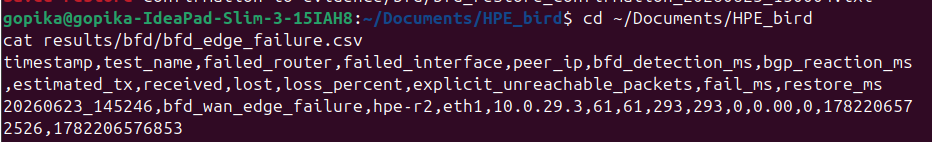
\includegraphics[width=0.95\textwidth]{../screenshots/bfd/01_bfd_detection_result_csv.png}
\caption{BFD detection result CSV}
\end{figure}

\begin{figure}[H]
\centering
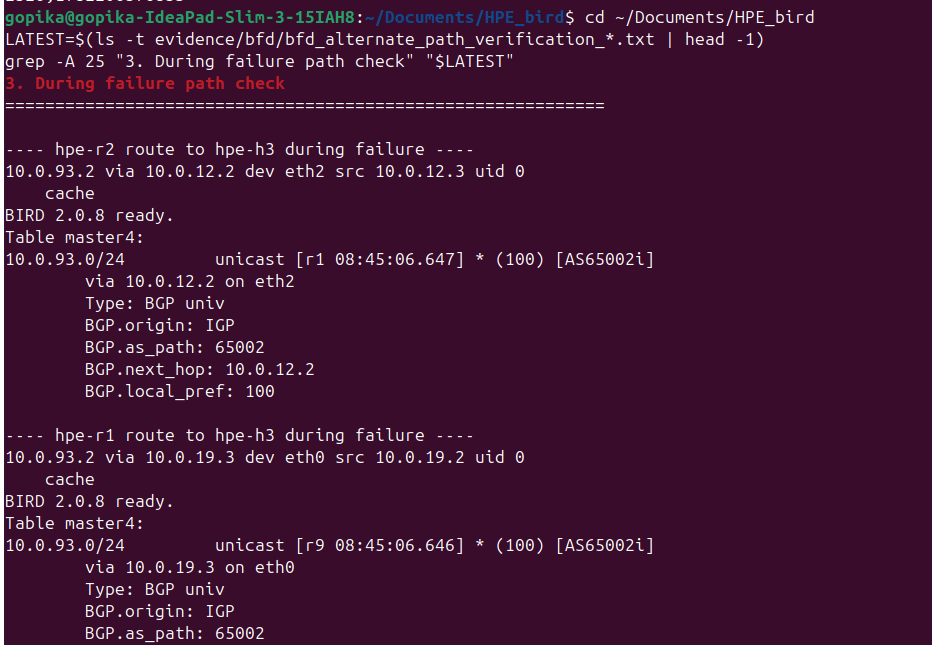
\includegraphics[width=0.95\textwidth]{../screenshots/bfd/02_bfd_alternate_path_during_failure.png}
\caption{BFD alternate path during failure}
\end{figure}

\begin{figure}[H]
\centering
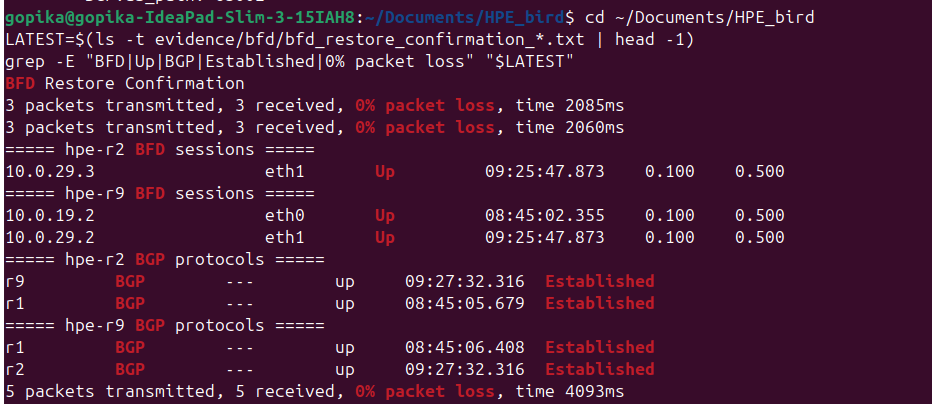
\includegraphics[width=0.95\textwidth]{../screenshots/bfd/03_bfd_restore_confirmation.png}
\caption{BFD restore confirmation}
\end{figure}

\begin{figure}[H]
\centering
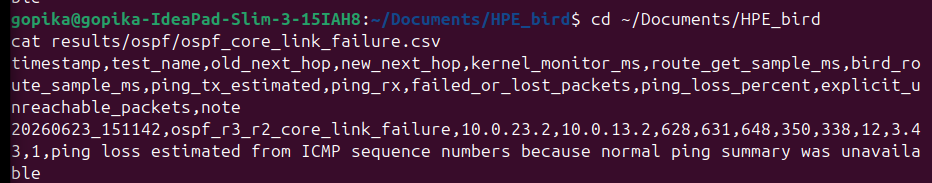
\includegraphics[width=0.95\textwidth]{../screenshots/ospf_core_failure/01_ospf_core_failure_csv.png}
\caption{OSPF core failure CSV}
\end{figure}

\begin{figure}[H]
\centering
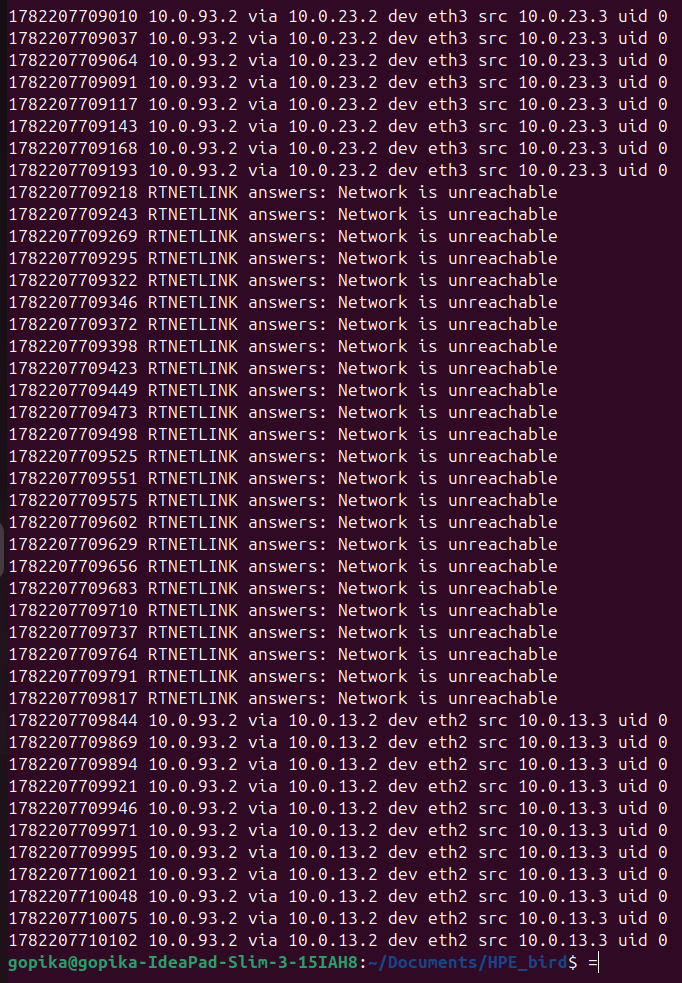
\includegraphics[width=0.95\textwidth]{../screenshots/ospf_core_failure/03_ospf_route_get_samples.png}
\caption{OSPF route sampling during recovery}
\end{figure}

\begin{figure}[H]
\centering
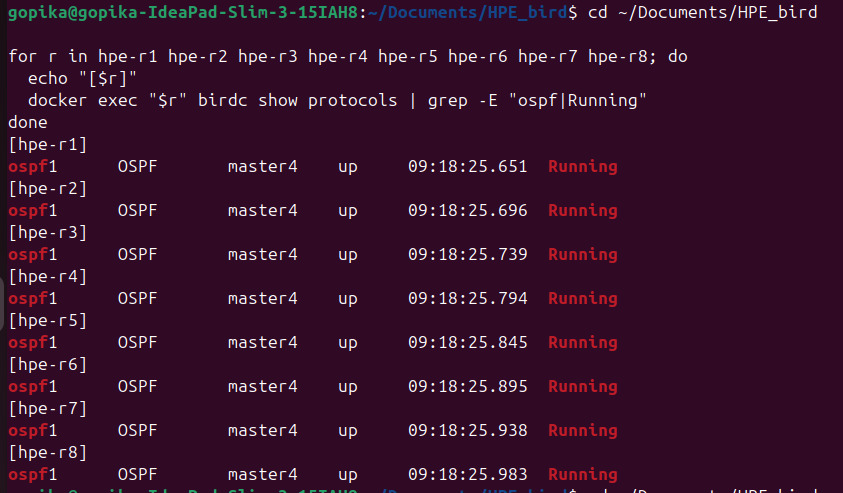
\includegraphics[width=0.95\textwidth]{../screenshots/ospf_core_failure/04_ospf_final_health.png}
\caption{OSPF final health}
\end{figure}

\begin{figure}[H]
\centering
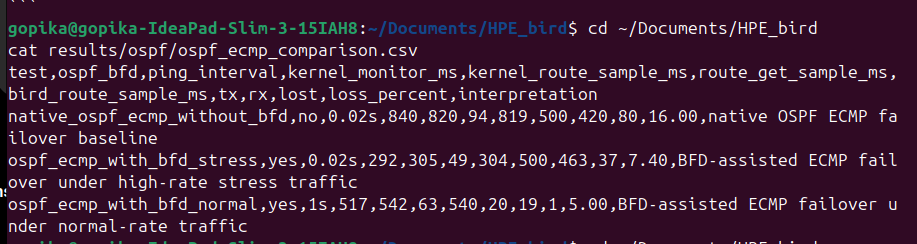
\includegraphics[width=0.95\textwidth]{../screenshots/ospf_ecmp/01_ospf_ecmp_comparison_csv.png}
\caption{OSPF ECMP comparison CSV}
\end{figure}

\begin{figure}[H]
\centering
\includegraphics[width=0.95\textwidth]{../screenshots/ospf_ecmp/02_ecmp_route_before_failure.png}
\caption{OSPF ECMP route before failure}
\end{figure}

\begin{figure}[H]
\centering
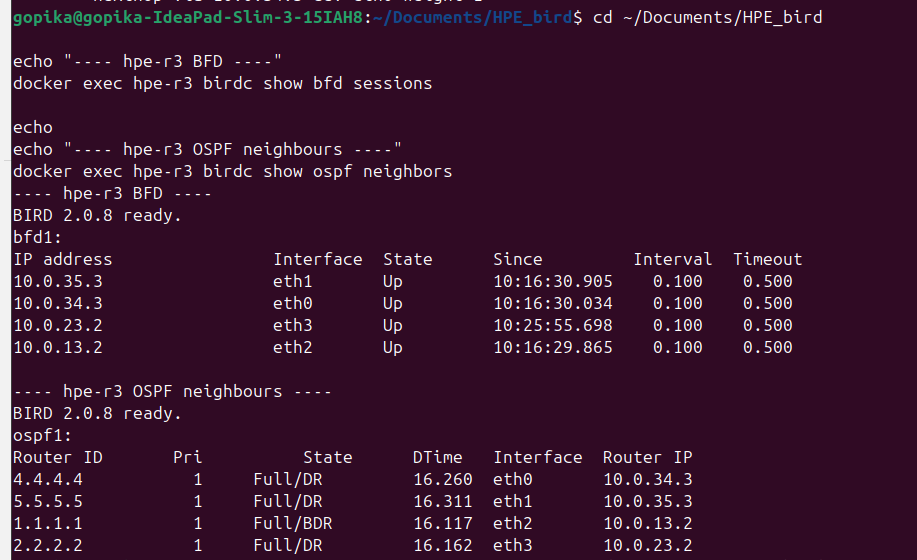
\includegraphics[width=0.95\textwidth]{../screenshots/ospf_ecmp/03_ospf_bfd_sessions_active.png}
\caption{OSPF-BFD sessions active}
\end{figure}

\begin{figure}[H]
\centering
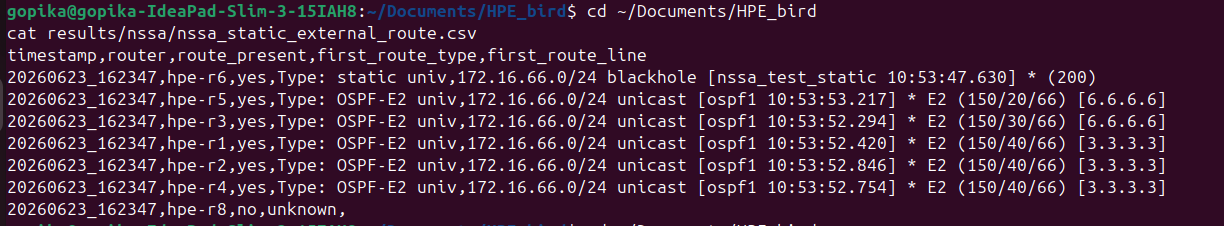
\includegraphics[width=0.95\textwidth]{../screenshots/nssa/01_nssa_type7_type5_csv.png}
\caption{NSSA Type-7 and Type-5 CSV}
\end{figure}

\begin{figure}[H]
\centering
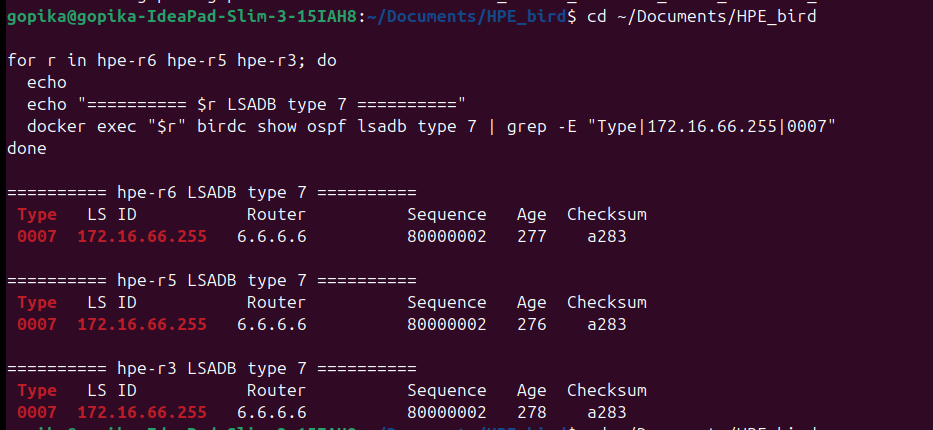
\includegraphics[width=0.95\textwidth]{../screenshots/nssa/02_type7_inside_nssa.png}
\caption{Type-7 LSA inside NSSA}
\end{figure}

\begin{figure}[H]
\centering
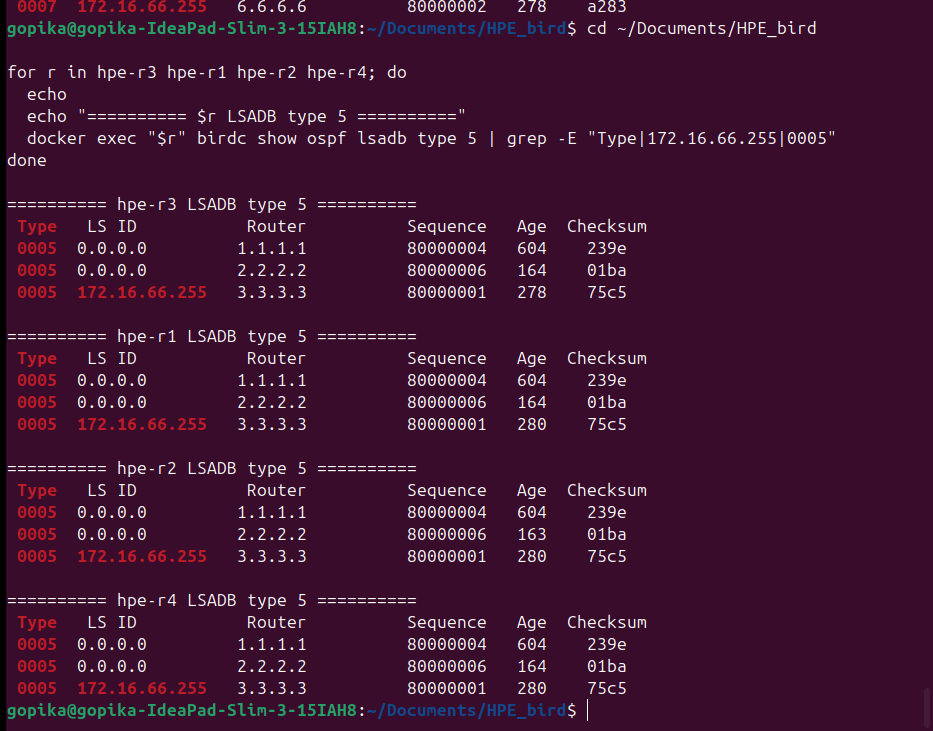
\includegraphics[width=0.95\textwidth]{../screenshots/nssa/03_type5_outside_nssa.png}
\caption{Type-5 LSA outside NSSA}
\end{figure}

\begin{figure}[H]
\centering
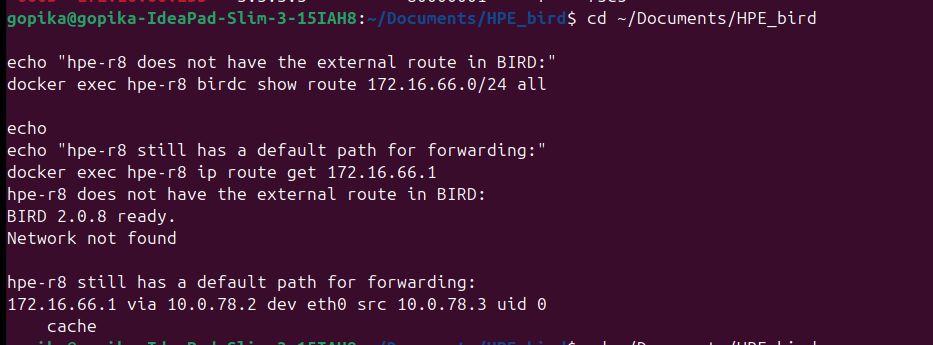
\includegraphics[width=0.95\textwidth]{../screenshots/nssa/04_stub_area_external_route_containment.png}
\caption{Stub area external route containment}
\end{figure}

\begin{figure}[H]
\centering
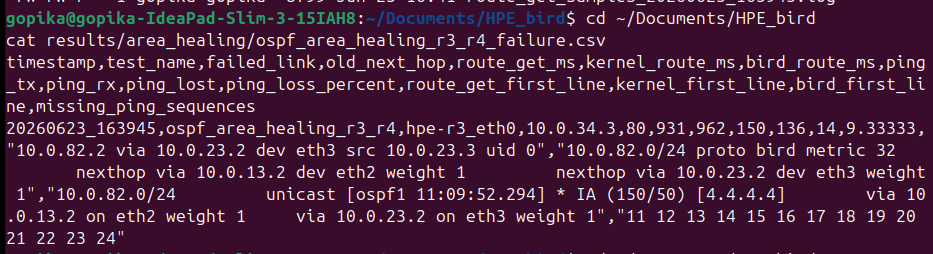
\includegraphics[width=0.95\textwidth]{../screenshots/area_healing/01_area_healing_csv.png}
\caption{OSPF area healing CSV}
\end{figure}

\begin{figure}[H]
\centering
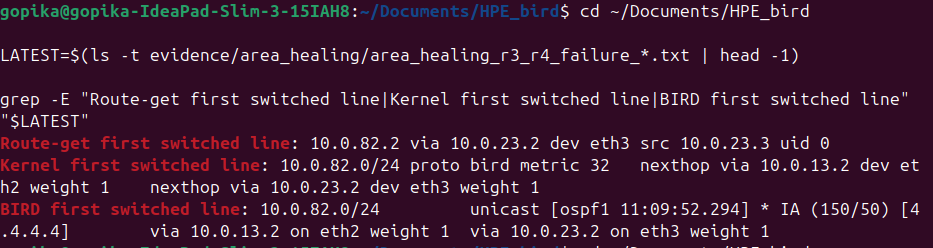
\includegraphics[width=0.95\textwidth]{../screenshots/area_healing/03_route_after_healing.png}
\caption{OSPF area route after healing}
\end{figure}

\begin{figure}[H]
\centering
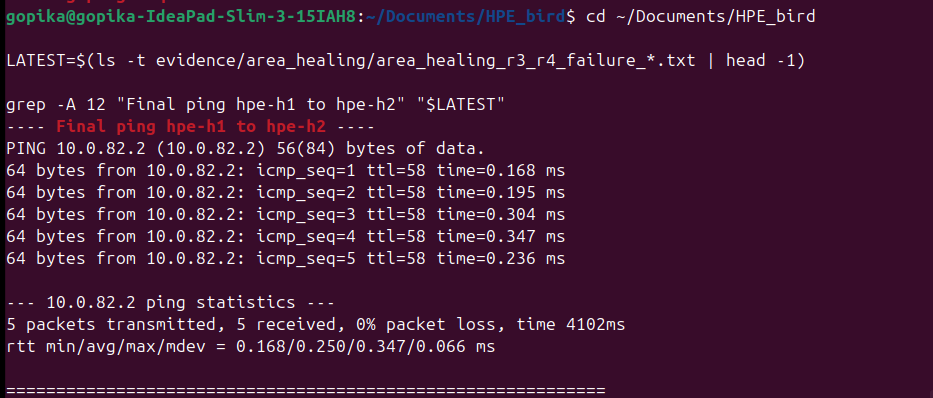
\includegraphics[width=0.95\textwidth]{../screenshots/area_healing/05_final_restored_health.png}
\caption{OSPF area final restored health}
\end{figure}

\begin{figure}[H]
\centering
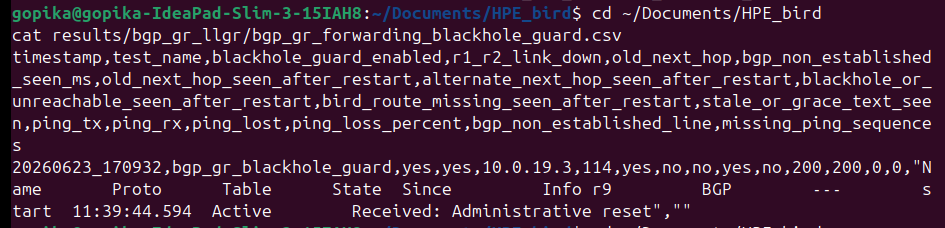
\includegraphics[width=0.95\textwidth]{../screenshots/bgp_gr_llgr/01_bgp_gr_blackhole_guard_csv.png}
\caption{BGP GR blackhole guard CSV}
\end{figure}

\begin{figure}[H]
\centering
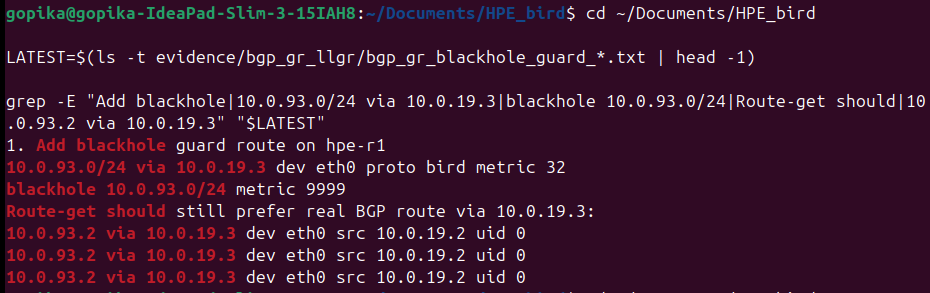
\includegraphics[width=0.95\textwidth]{../screenshots/bgp_gr_llgr/02_blackhole_guard_real_route_preferred.png}
\caption{BGP GR blackhole guard real route preferred}
\end{figure}

\begin{figure}[H]
\centering
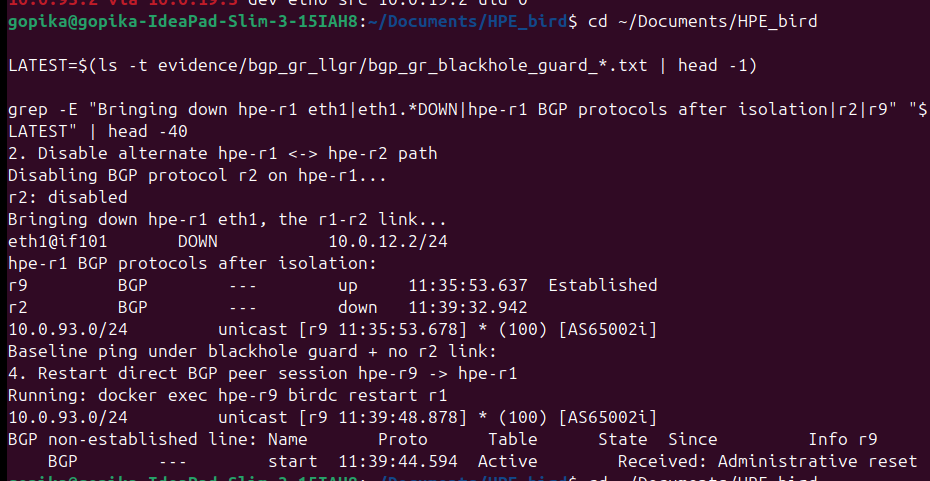
\includegraphics[width=0.95\textwidth]{../screenshots/bgp_gr_llgr/03_alternate_path_disabled.png}
\caption{BGP alternate path disabled}
\end{figure}

\begin{figure}[H]
\centering
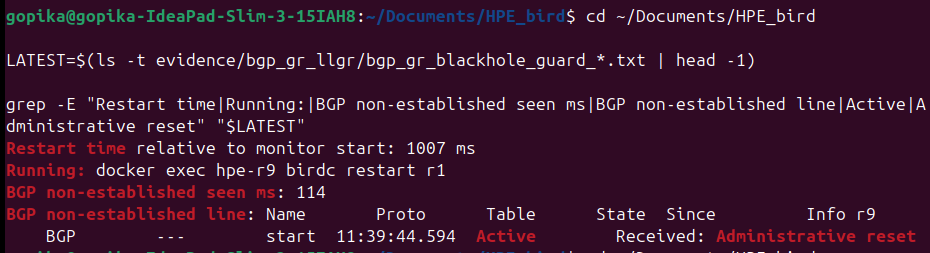
\includegraphics[width=0.95\textwidth]{../screenshots/bgp_gr_llgr/04_bgp_restart_observed.png}
\caption{BGP restart observed}
\end{figure}

\begin{figure}[H]
\centering
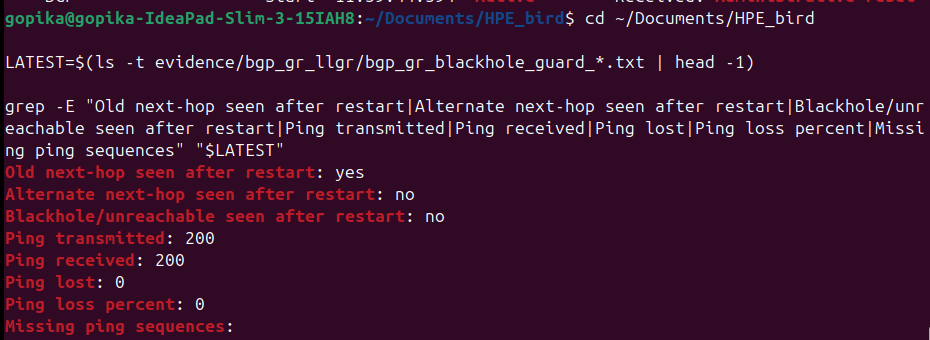
\includegraphics[width=0.95\textwidth]{../screenshots/bgp_gr_llgr/05_forwarding_continued_no_fallback.png}
\caption{BGP forwarding continued without fallback}
\end{figure}

\begin{figure}[H]
\centering
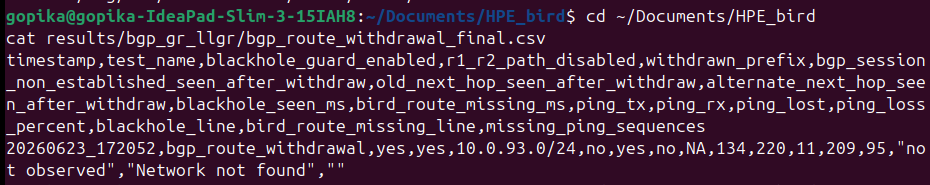
\includegraphics[width=0.95\textwidth]{../screenshots/bgp_gr_llgr/06_bgp_withdrawal_csv.png}
\caption{BGP withdrawal CSV}
\end{figure}

\begin{figure}[H]
\centering
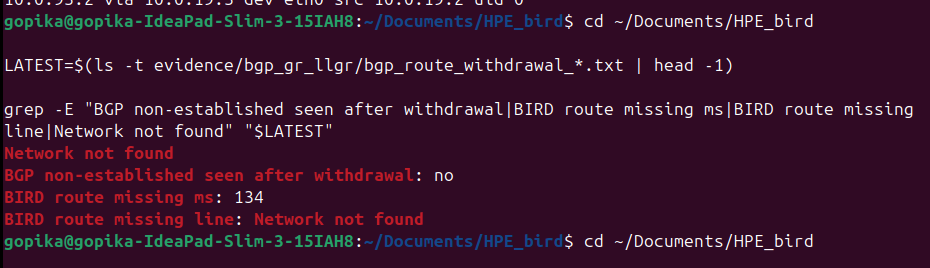
\includegraphics[width=0.95\textwidth]{../screenshots/bgp_gr_llgr/08_route_withdrawn_bgp_still_up.png}
\caption{BGP route withdrawn while session stayed up}
\end{figure}

\begin{figure}[H]
\centering
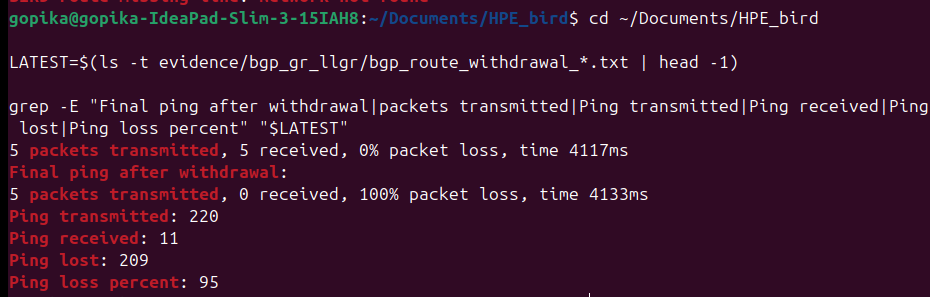
\includegraphics[width=0.95\textwidth]{../screenshots/bgp_gr_llgr/09_withdrawal_packet_loss.png}
\caption{BGP withdrawal packet loss}
\end{figure}

% --- NEW DELIVERABLE TERMINAL SCREENSHOTS START ---

\subsection{Additional Deliverable Terminal Evidence}

The following screenshots show terminal evidence for the additional deliverable experiments: multi-hop BFD, BGP full daemon restart, and BGP peer flap recovery.

\begin{figure}[H]
\centering
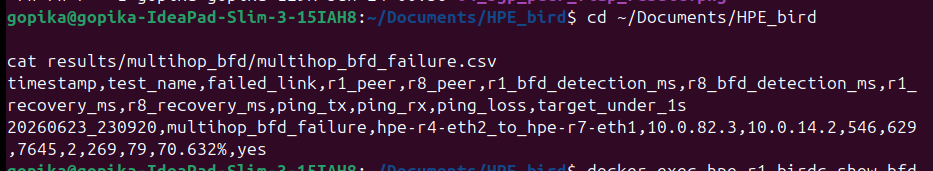
\includegraphics[width=0.95\textwidth]{../screenshots/new_deliverables_terminal/01_multihop_bfd_sessions.png}
\caption{01 multihop bfd sessions}
\end{figure}

\begin{figure}[H]
\centering
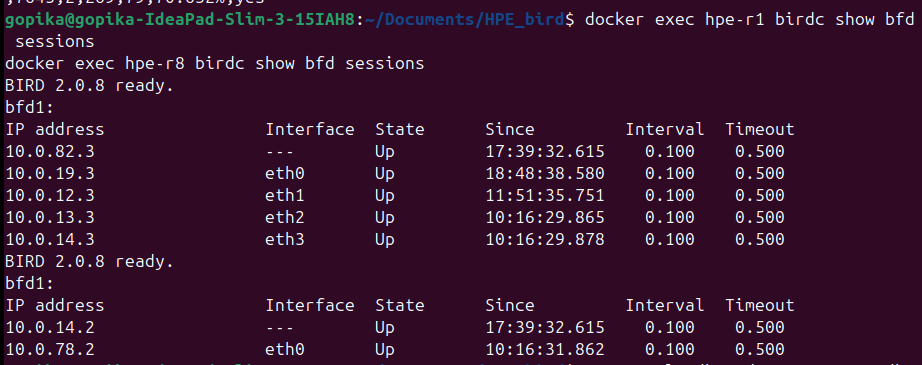
\includegraphics[width=0.95\textwidth]{../screenshots/new_deliverables_terminal/02_multihop_bfd_result_csv.png}
\caption{02 multihop bfd result csv}
\end{figure}

\begin{figure}[H]
\centering
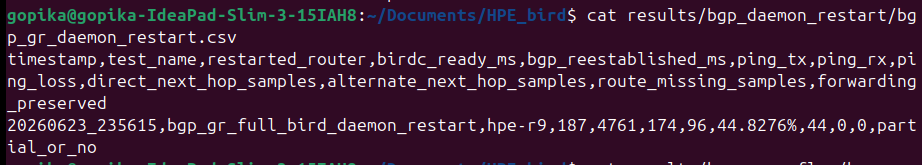
\includegraphics[width=0.95\textwidth]{../screenshots/new_deliverables_terminal/03_bgp_daemon_restart_result_csv.png}
\caption{03 bgp daemon restart result csv}
\end{figure}

\begin{figure}[H]
\centering
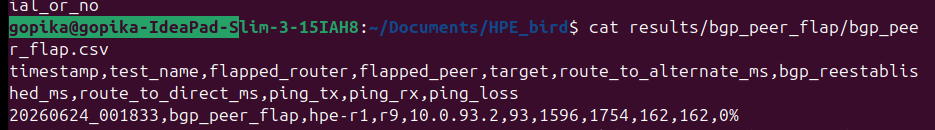
\includegraphics[width=0.95\textwidth]{../screenshots/new_deliverables_terminal/04_bgp_peer_flap_result_csv.png}
\caption{04 bgp peer flap result csv}
\end{figure}

% --- NEW DELIVERABLE TERMINAL SCREENSHOTS END ---

\begin{figure}[H]
\centering
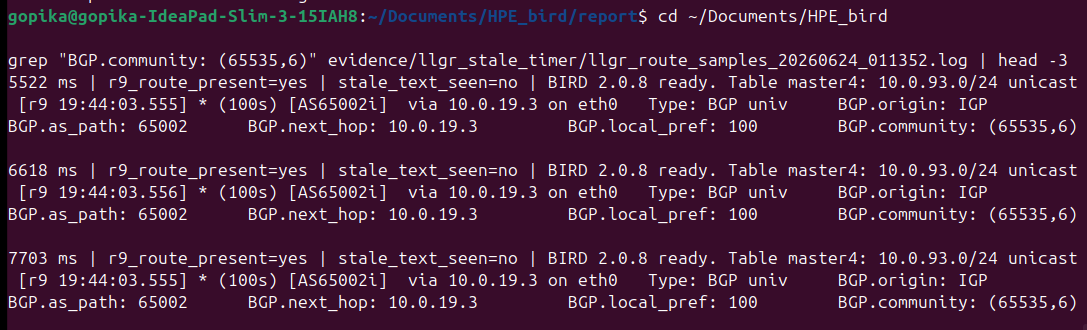
\includegraphics[width=0.95\textwidth]{../screenshots/new_deliverables_terminal/05_llgr_stale_marker.png}
\caption{LLGR stale route marker shown as \texttt{(100s)} and \texttt{BGP.community: (65535,6)}}
\end{figure}

